\documentclass[
aspectratio=1610,
hyperref={pdfpagemode=FullScreen},
english,
usenames,
dvipsnames
]
{beamer} %If you want to create Polish presentation, replace 'english' with 'polish'

\usepackage[utf8]{inputenc}
\usepackage{polski} %For Polish language only
\usepackage[T1]{fontenc}
\usepackage{verbatim}
\usepackage[usefamily=bash]{pythontex}
\usepackage{listings} %We want to put listings


\usetheme[parttitle=rightfooter]{AGH} %Show part title in right footer
%\usetheme[dark]{AGH}                 %Use dark background
%\usetheme[dark,parttitle=leftfooter]{AGH}  %Use dark background and show part title in left footer

\AtBeginPart{\frame{\partpage}} %At begin part: display its name
\title{Python\TeX}
\author{Damian Łączak}
\date{}
\institute[AGH]{
Edycja i prezentacja tekstów naukowych \\
\pyc{import sys}
Python: \py{sys.version}
}
%%%%%%%%%%% Configuration of the listings package %%%%%%%%%%%%%%%%%%%%%%%%%%
% Source: https://en.wikibooks.org/wiki/LaTeX/Source_Code_Listings#Using_the_listings_package
%%%%%%%%%%%%%%%%%%%%%%%%%%%%%%%%%%%%%%%%%%%%%%%%%%%%%%%%%%%%%%%%%%%%%%%%%%%%
\lstset{ %
  backgroundcolor=\color{white},   % choose the background color
  basicstyle=\footnotesize,        % the size of the fonts that are used for the code
  breakatwhitespace=false,         % sets if automatic breaks should only happen at whitespace
  breaklines=true,                 % sets automatic line breaking
  captionpos=b,                    % sets the caption-position to bottom
  commentstyle=\color{ForestGreen},      % comment style
  deletekeywords={...},            % if you want to delete keywords from the given language
  escapeinside={\%*}{*)},          % if you want to add LaTeX within your code
  extendedchars=true,              % lets you use non-ASCII characters; for 8-bits encodings only, does not work with UTF-8
  frame=single,	                   % adds a frame around the code
  keepspaces=true,                 % keeps spaces in text, useful for keeping indentation of code (possibly needs columns=flexible)
  keywordstyle=\color{blue},       % keyword style
  morekeywords={*,...},            % if you want to add more keywords to the set
  numbers=left,                    % where to put the line-numbers; possible values are (none, left, right)
  numbersep=5pt,                   % how far the line-numbers are from the code
  numberstyle=\tiny\color{gray}, % the style that is used for the line-numbers
  rulecolor=\color{black},         % if not set, the frame-color may be changed on line-breaks within not-black text (e.g. comments (green here))
  showspaces=false,                % show spaces everywhere adding particular underscores; it overrides 'showstringspaces'
  showstringspaces=false,          % underline spaces within strings only
  showtabs=false,                  % show tabs within strings adding particular underscores
  stepnumber=1,                    % the step between two line-numbers. If it's 1, each line will be numbered
  stringstyle=\color{cyan},        % string literal style
  tabsize=2,	                   % sets default tabsize to 2 spaces
  belowskip=0em,
  title=\lstname,                  % show the filename of files included with \lstinputlisting; also try caption instead of title
                                   %  needed if you want to use UTF-8 Polish chars
  literate={ą}{{\k{a}}}1
           {Ą}{{\k{A}}}1
           {ę}{{\k{e}}}1
           {Ę}{{\k{E}}}1
           {ó}{{\'o}}1
           {Ó}{{\'O}}1
           {ś}{{\'s}}1
           {Ś}{{\'S}}1
           {ł}{{\l{}}}1
           {Ł}{{\L{}}}1
           {ż}{{\.z}}1
           {Ż}{{\.Z}}1
           {ź}{{\'z}}1
           {Ź}{{\'Z}}1
           {ć}{{\'c}}1
           {Ć}{{\'C}}1
           {ń}{{\'n}}1
           {Ń}{{\'N}}1
}
%%%%%%%%%%%%%%%%%

%%%%%moje zmianki



\begin{document}
  \maketitle
\part{Basics of Python\TeX}
%%%%%%%%%%%%%%%%
\begin{frame}{Outline}
	\tableofcontents[
	pausesections,
	currentsubsection, 
	hideothersubsections, 
	sectionstyle=show, 
	subsectionstyle=show
	]
\end{frame}
%%%%%%%%%%%%%%%%
\section{Python basics}
\subsection{First example}
%%%%%%%%%%%%%%%%
  \begin{frame}[fragile]{First example}{No brackets only indentation}
    \begin{lstlisting}[language=python]
# And this is a comment.
from random import randint
number = randint(0, 9)
if number < 5:
    print("0-4")
else:
    print("5-9")
 
\end{lstlisting}
\begin{exampleblock}{Example output}
    0-4
    \onslide
\end{exampleblock}

\end{frame}
\subsection{Functions}
\begin{frame}[fragile]{Functions}
    \begin{lstlisting}[language=python]
def sayMyName(name):
    print ("Your name is {0}".format(name))
sayMyName("Damian")
\end{lstlisting}

\begin{exampleblock}{Output}
    Your name is Damian
     \onslide
\end{exampleblock}
\end{frame}
%%%%%%%%%%%%%%%%

%%%%%%%%%%%%%%%%
\section{Compilation process}
\subsection{Outline}
%%%%%%%%%%%%%%%%
\begin{frame}{PDF creation process}
	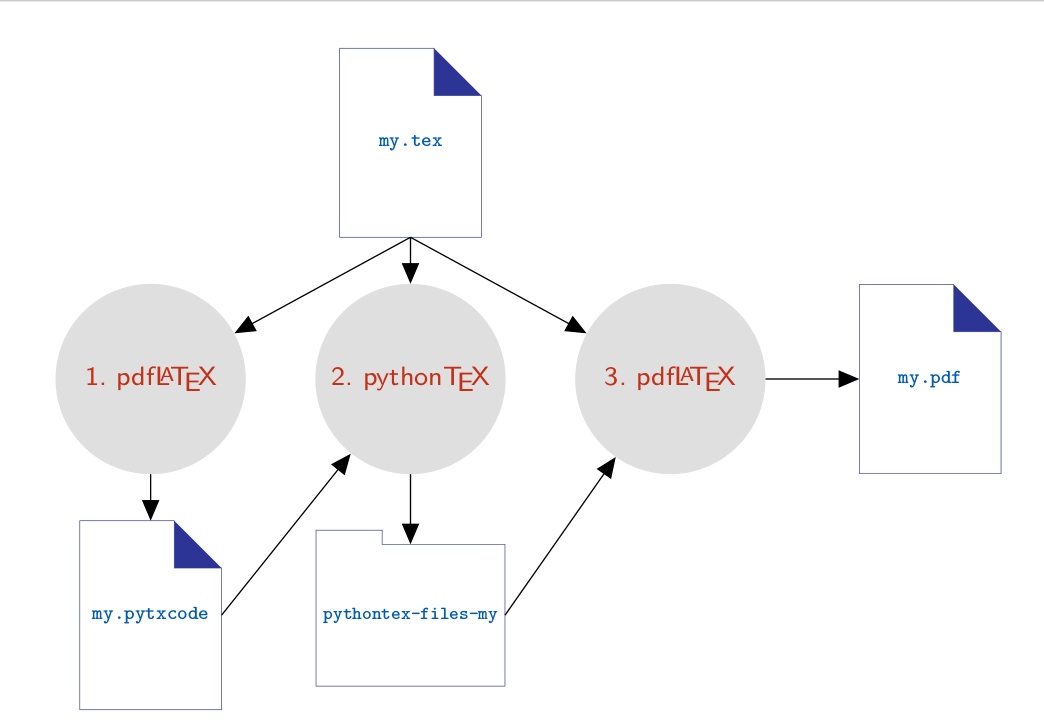
\includegraphics[scale=0.25]{img/compile.png}
\end{frame}
\section{Python\TeX}
\subsection{Sessions}
  \begin{frame}[fragile]{Sessions}{What are they for?}
  \begin{itemize}[<+->]
  \item Parallel execution
  	\begin{itemize}
  		\item Increase speed
  		\item Different settings
  	\end{itemize}
  \item Default session
  \item Session name
  	\begin{itemize}
  		\item a-z
  		\item A-Z
  		\item 0-9
  		\item hyphen and underscore
  		 \onslide
  	\end{itemize}
  \end{itemize}
\end{frame}

\subsection{Commands}
  \begin{frame}{Commands}{Overall look on them}
  	\begin{columns}
  	\column{0.33\textwidth}
  	Inline commands
  	\begin{itemize}
  		\item py
  		\item pyc
  		\item pys
  		\item pyv
  		\item pyb
  	\end{itemize}
  	\column{0.33\textwidth}
  	Multi-line commands
  	\begin{itemize}
  		\item pycode
  		\item pysub
  		\item pyverbatim
  		\item pyblock
  	\end{itemize}
  	\column{0.33\textwidth}
  	Console commands
  	\begin{itemize}
  		\item pyconsole
  		\item pycon
  	\end{itemize}
  	\onslide
  	\end{columns}
  \end{frame}
  \begin{frame}[fragile]{py}{inline command}
  
  \begin{block}{Usage}
  	Returns text representation  of it's argument.
  \end{block}
  
  \begin{lstlisting}[language=python]
	\py{"Hello world"}
  \end{lstlisting}
  
  	\begin{exampleblock}{output}
\py{"Hello world"}
    \onslide
	\end{exampleblock}
  
  \end{frame}
  
  \begin{frame}[fragile]{pyc}{inline command}
  
  \begin{block}{Usage}
  	Prints evaluated expressions that are inside curly braces preceded by exclamation mark.
  \end{block}
  
  \begin{lstlisting}[language=python]
\pyc{a = 2**8}
\py{a}
  \end{lstlisting}
  
  	\begin{exampleblock}{output}
    \pyc{a = 2**8}
	\py{a}
    \onslide
	\end{exampleblock}
  
  \end{frame}
  
\begin{frame}[fragile]{pys}{inline command}
  
  \begin{block}{Usage}
  Evaluates and then substitute expressions that are surrounded by curly braces proceeded by exclamation mark by their string representation. 
  \end{block}
  
  \begin{lstlisting}[language=python]
\pys{$1 + 1 = !{1+1}$}
  \end{lstlisting}
  
  	\begin{exampleblock}{output}
    \pys{$1 + 1 = !{1+1}$}
    \onslide
	\end{exampleblock}
  
  \end{frame}
  
  \begin{frame}[fragile]{pyv}{inline command}
  
  \begin{block}{Usage}
  	It typesets but do not execute the code. 
  \end{block}
  
  \begin{lstlisting}[language=python]
\pyc{a = 1}
\pyv{a = 256} \\
\py{a}
  \end{lstlisting}
  
  	\begin{exampleblock}{output}
    \pyc{a = 1}
\pyv{a = 256} \\
\py{a}
    \onslide
	\end{exampleblock}
  
  \end{frame}
  
  
   \begin{frame}[fragile]{pyb}{inline command}
  
  \begin{block}{Usage}
  	It typesets and executes the code. 
  \end{block}
  
  \begin{lstlisting}[language=python]
\pyc{a = 1}
\pyb{a = 256} \\
\py{a}
  \end{lstlisting}
  
  	\begin{exampleblock}{output}
    \pyc{a = 1}
\pyb{a = 256} \\
\py{a}
    \onslide
	\end{exampleblock}
  
  \end{frame}
  
  \begin{frame}[fragile]{pycode}{environment}
  
  \begin{block}{Usage}
  	Enclose the code that is going to be executed but not typeset.
  \end{block}
  
  \begin{lstlisting}[language=python]
\begin{pycode}
def sayMyName(name):
	return "Your name is {0}".format(name)
sayMyName("Damian")  
\end{pycode}
\py{sayMyName("Damian")}
  \end{lstlisting}
  
  	\begin{exampleblock}{output}
\begin{pycode}
def sayMyName(name):
	return "Your name is {0}".format(name)
sayMyName("Damian")  
\end{pycode}
\py{sayMyName("Damian")}
    \onslide
	\end{exampleblock}
  
  \end{frame}
  
    \begin{frame}[fragile]{pysub}{environment}
  
  \begin{block}{Usage}
  	Similar to $\textbackslash$pys. But this time this is an environment.
  \end{block}
  
  \begin{lstlisting}[language=python]
\begin{pysub}
1 + 5 = !{1 + 5} \\
Function output: !{sayMyName("Damian")} \\
2*32 = !{2**32}
\end{pysub}
  \end{lstlisting}
  
  	\begin{exampleblock}{output}
\begin{pysub}
1 + 5 = !{1 + 5} \\
Function output: !{sayMyName("Damian")} \\
2*32 = !{2**32}
\end{pysub}
    \onslide
	\end{exampleblock}
  
  \end{frame}
  
    \begin{frame}[fragile]{pyblock}{environment}
  
  \begin{block}{Usage}
  	This environment enclose the code that is typeset and executed.
  	Does not print any printed content even if autoprint flag is set to true.
  \end{block}
  
 \begin{lstlisting}[language=python]
\begin{pyblock}
sayMyName("Damian")
a = 125
a + a
\end{pyblock}
  \end{lstlisting}
  
  	\begin{exampleblock}{output}
\begin{pyblock}
sayMyName("Damian")
a = 125
a + a
\end{pyblock}
    \onslide
	\end{exampleblock}
  
  \end{frame}  
  
      \begin{frame}[fragile]{pyverbatim}{environment}
  
  \begin{block}{Usage}
  	This environment enclose the code that is typeset and not executed.
  \end{block}
  
 \begin{lstlisting}[language=python]
\begin{pyverbatim}
sayMyName("Damian")
a = 125
a + a
\end{pyverbatim}
  \end{lstlisting}
  
  	\begin{exampleblock}{output}
\begin{pyverbatim}
sayMyName("Damian")
a = 125
a + a
\end{pyverbatim}
    \onslide
	\end{exampleblock}
  
  \end{frame} 
  
   \begin{frame}[fragile]{pyconsole}{console environment}
  
  \begin{block}{Usage}
  	This environment treats its contents as series of commands passed to an active Python console. It shows input and output of commands.
  \end{block}
  
 \begin{lstlisting}[basicstyle=\tiny, language=python]
\begin{pyconsole}
a = [1, 2, 3] 
dir(a) 
print(a)
\end{pyconsole}
\end{lstlisting}
  
\begin{exampleblock}{output}
\begin{pyconsole}
a = [1, 2, 3]
dir(a)
print(a)
\end{pyconsole}
    \onslide
	\end{exampleblock}
  
  \end{frame}
  
  \begin{frame}[fragile]{pycon}{console inline command}
  
  \begin{block}{Usage}
  	This command executes code using emulated interpreter and shows the output back into the document, discarding the input.
  \end{block}
  
 \begin{lstlisting}[basicstyle=\tiny, language=python]
\pycon{dir(a)}
\end{lstlisting}
  
\begin{exampleblock}{output}
\pycon{dir(a)}
    \onslide
	\end{exampleblock}
  
  \end{frame}

\subsection{Other commands/functions}
\begin{frame}[fragile]{Other commands or functions}{Which are not so important to have single slide for them.}

\begin{itemize}[<+->]
\item \textbackslash{}setpythontexoutputdir
\item \textbackslash{}setpythontexworkingdir
\item str
\item add\_dependencies
\item before
\item after
\end{itemize}
\onslide
\end{frame}
\subsection{Beamer compatibility}
\begin{frame}{Beamer}
\begin{center}
	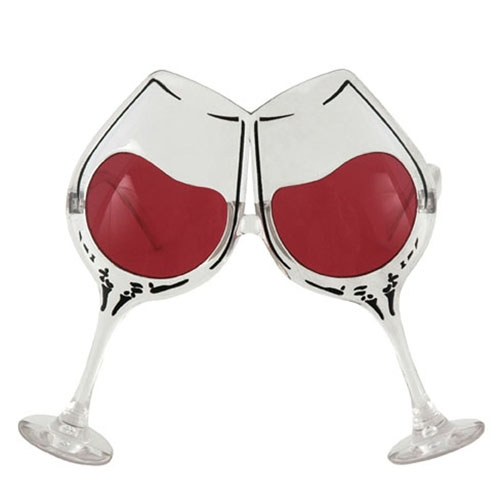
\includegraphics[scale=0.3, keepaspectratio]{hurra.jpg}
	\begin{alertblock}{Frames}
		Pyton\TeX \hspace{1pt} is compatible with Beamer. But beware, you need to use Beamer's fragile option for any frame containing typeset code.
	\end{alertblock}
\end{center}
\end{frame}

\subsection{Other languages}
\begin{frame}[fragile]{Other languages}
  \begin{itemize}[<+->]
  \item Ruby
  \item Octave
  \item Julia
  \item Rust
  \item Bash
  \end{itemize}
\end{frame}

\begin{frame}[fragile]{Bash}{Available commands and environments}
  \begin{itemize}[<+->]
  \item bash
  \item bashblock
  \item bashverbatim
  \item bashsub
  \end{itemize}
\end{frame}


\part{Python \TeX{}amples}

\begin{frame}{Outline}
	\tableofcontents[
	pausesections,
	currentsubsection, 
	hideothersubsections, 
	sectionstyle=show, 
	subsectionstyle=show
	]
	\onslide
\end{frame}

\section{Charts}
\subsection{source code}
\begin{frame}[fragile]{Chart}{Matplotlib}
\begin{lstlisting}[language=python]
\begin{pycode}[chart]
from pylab import *
def f(t):
    return cos(2 * pi * t) * exp(-t)
t = linspace(0, 5, 500)
y = f(t)
clf()
figure(figsize=(5, 3))
rc("text", usetex=True)
plot(t, y)
title("Przykladowy wykres")
text(3, 0.15, r"$y = \cos(2 \pi t) e^{-t}$")
xlabel("czas (s)")
ylabel("napiecie (mV)")
savefig("myplot.png", bbox_inches="tight")
print(r"\begin{center}")
print(r"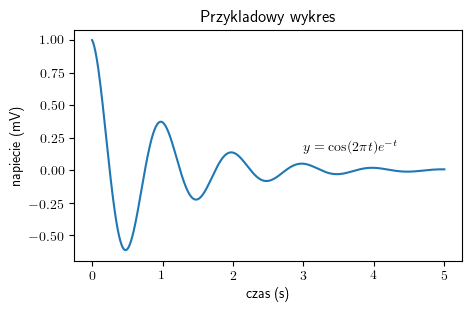
\includegraphics[scale=1.0, keepaspectratio]{myplot.png}")
print(r"\end{center}")
\end{pycode}
\end{lstlisting}
\end{frame}
\subsection{result}
\begin{frame}[fragile]{Chart}{File is saved to main folder by default}
\begin{pycode}[chart]
from pylab import *
def f(t):
    return cos(2 * pi * t) * exp(-t)
t = linspace(0, 5, 500)
y = f(t)
clf()
figure(figsize=(5, 3))
rc("text", usetex=True)
plot(t, y)
title("Przykladowy wykres")
text(3, 0.15, r"$y = \cos(2 \pi t) e^{-t}$")
xlabel("czas (s)")
ylabel("napiecie (mV)")
savefig("myplot.png", bbox_inches="tight")
print(r"\begin{center}")
print(r"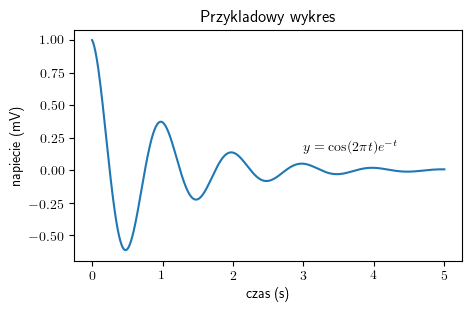
\includegraphics[scale=1.0, keepaspectratio]{myplot.png}")
print(r"\end{center}")
\end{pycode}
\end{frame}


\section{Internet data}
\subsection{source code}
\begin{frame}[fragile]{GPW}{Using another session to improve speed of pythontex.}
\begin{lstlisting}[language=python]
\begin{pycode}[internet]
from internet import getSymbolInfo
import time

wig20 = getSymbolInfo("WIG20")
kghm = getSymbolInfo("KGHM")
cd = getSymbolInfo("CDPROJEKT")
date = time.strftime("%Y/%m/%d");
\end{pycode}

\begin{exampleblock}{KGHM}
Current price: \py[internet]{wig20} PLN
\end{exampleblock}

\end{lstlisting}
\end{frame}
\subsection{result}
\begin{frame}[fragile]{GPW}{Because it's funny to know the current price of stock.}
\begin{pycode}[internet]
from internet import getSymbolInfo
import time

wig20 = getSymbolInfo("WIG20")
kghm = getSymbolInfo("KGHM")
cd = getSymbolInfo("CDPROJEKT")
date = time.strftime("%Y/%m/%d");
\end{pycode}


\begin{exampleblock}{WIG20}
Current price: \py[internet]{wig20}
\end{exampleblock}

\begin{exampleblock}{KGHM}
Current price: \py[internet]{kghm} PLN
\end{exampleblock}

\begin{exampleblock}{CDPROJEKT}
Current price: \py[internet]{cd} PLN
\end{exampleblock}

Actual price for date: \py[internet]{date}.

\onslide
\end{frame}

\section{Dynamic tables}
\subsection{source code}
\begin{frame}[fragile]{External files}
\begin{lstlisting}[language=python]
\begin{pycode}[people]
from people import importPeople
people = importPeople()	

print(r"\begin{tabular}{ l | r }")

print(r"{0} & {1} \\ \hline".format(people[0][0], people[0][1]))
people.pop(0)
for person in people:
	print(r"{0} & {1} \\".format(person[0], person[1]))
	
print(r"\end{tabular}")
\end{pycode}

\end{lstlisting}
\end{frame}
\subsection{result}
\begin{frame}[fragile]{External files}{The biggest hassle of creating tables is finally diminished.}
\begin{exampleblock}{List of people}
\begin{pycode}[people]
from people import importPeople
people = importPeople()	
print(r"\begin{tabular}{ l | r }")
print(r"{0} & {1} \\ \hline".format(people[0][0], people[0][1]))
people.pop(0)
for person in people:
	print(r"{0} & {1} \\".format(person[0], person[1]))
print(r"\end{tabular}")
\end{pycode}
\end{exampleblock}

\onslide
\end{frame}

\appendix
\begin{frame}[allowframebreaks]{Bibliography}
  \begin{thebibliography}{9}
    \setbeamertemplate{bibliography item}[online]
      \bibitem{wikibook}{CTAN \newblock Python\TeX \hspace{1pt} Package documentation \newblock \url{http://piotrkosoft.net/pub/mirrors/CTAN/macros/latex/contrib/pythontex/pythontex.pdf}}
      \setbeamertemplate{bibliography item}[online]
      \bibitem{wikibook}{CTAN \newblock Beamer user guide \newblock \url{http://mirrors.ctan.org/macros/latex/contrib/beamer/doc/beameruserguide.pdf}}
  \end{thebibliography}
\end{frame}
\end{document}

